\chapter{Results}
\label{sec:results}

\section{Findings from the Simulations}
As observed in preliminary tests, the QE scheme produces numerical errors, which manifest as repeated price values within the simulation. In a correctly executed simulation, the most frequently occurring price in the first simulated path appears only a few times. However, in cases where errors occur, this number increases to the hundreds or even thousands.

Figure \ref{fig:max_number_of_same_prices_distribution} illustrates the distribution of this phenomenon. The peak at 1 indicates that most simulations were performed correctly. However, the presence of cases where the same price appears up to 250,000 times suggests significant numerical instabilities. A closer examination of these faulty simulations reveals that once a numerical error occurs for the first time, the remaining time series retains the same price value throughout. In extreme cases where the same price appears 250,000 times, the error must have occurred very early in the simulation.

\begin{figure}
    \centering
    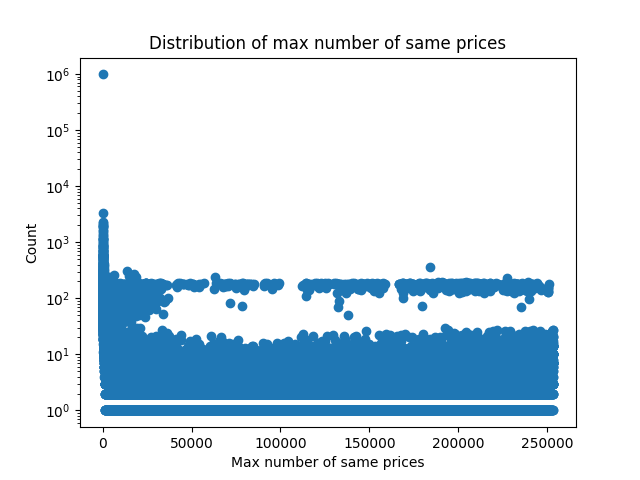
\includegraphics[width=0.8\textwidth]{img/max_number_of_same_prices_distribution.png}
    \caption{Distribution of the maximum number of the same prices in the first path of the simulation}
    \label{fig:max_number_of_same_prices_distribution}
\end{figure}

To ensure the reliability of the analysis, simulations exhibiting numerical errors will be excluded, as they are not correctly executed. However, since it is possible for identical prices to occur naturally in correct simulations, a threshold must be determined that retains as many valid simulations as possible while filtering out erroneous ones.

Figure \ref{fig:max_number_of_same_prices_cumulative_percentage} illustrates the cumulative percentage of simulations that do not exceed a given threshold for the maximum number of identical price occurrences. If the threshold is set to 1 -— meaning only simulations where no price ever appears more than once are retained —- 68.40\% of the simulations remain. Increasing the threshold reduces the number of discarded simulations, but at the cost of potentially including simulations with numerical errors. However, the impact is minimal, as the increase in retained simulations is negligible beyond a certain point.

For the final analysis, all simulations where any price appears more than once will be excluded to ensure data integrity.

\begin{figure}
    \centering
    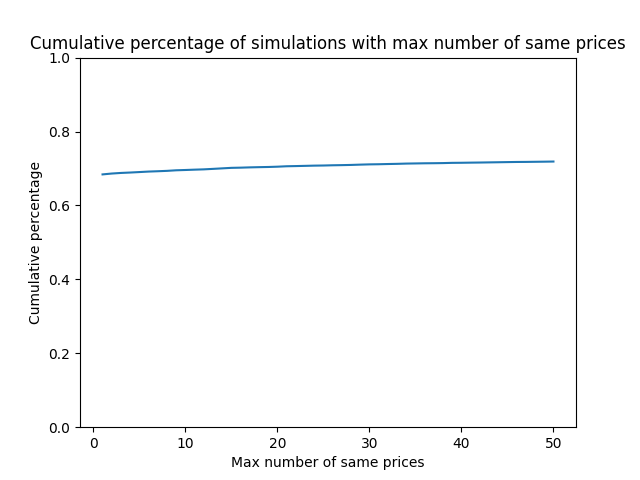
\includegraphics[width=0.8\textwidth]{img/max_number_of_same_prices_cumulative_percentage.png}
    \caption{Cumulative percentage of simulations that do not exceed the maximum number of same prices}
    \label{fig:max_number_of_same_prices_cumulative_percentage}
\end{figure}

\begin{figure}
    \centering
    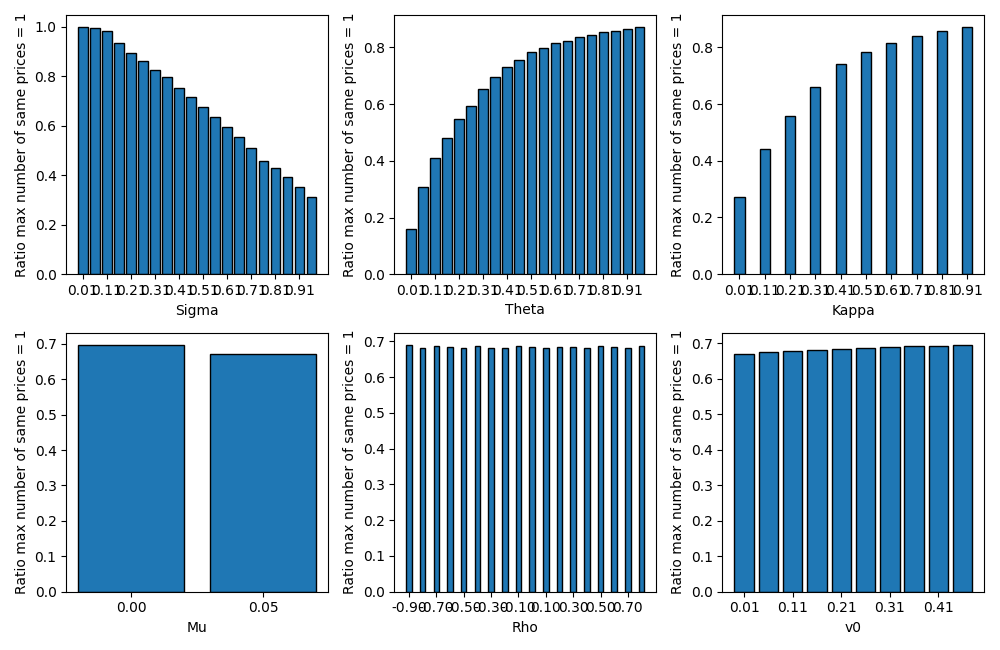
\includegraphics[width=0.8\textwidth]{img/max_number_of_same_prices_ratio_parameters.png}
    \caption{Ratio of simulations that do not exceed the maximum number of same prices in relation to the parameters of the Heston model}
    \label{fig:max_number_of_same_prices_ratio_parameters}
\end{figure}

\begin{figure}
    \centering
    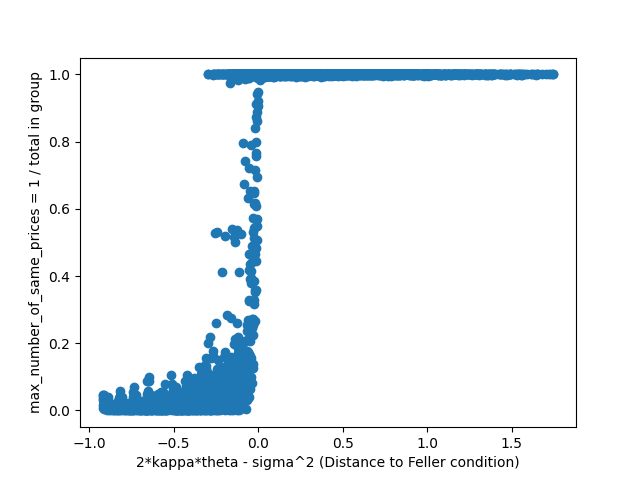
\includegraphics[width=0.8\textwidth]{img/max_number_of_same_prices_ratio_feller_diff.png}
    \caption{Ratio of simulations that do not exceed the maximum number of same prices in relation to the value $D$}
    \label{fig:max_number_of_same_prices_ratio_D}
\end{figure}

To analyze the source of these numerical errors, we examine the proportion of correct simulations as a function of each individual Heston model parameter (see Figure \ref{fig:max_number_of_same_prices_ratio_parameters}). The results show that as $\sigma$ increases, the error rate rises, whereas increasing $\theta$ and $\kappa$ reduces the frequency of errors. In contrast, the parameters $\mu$, $\rho$, and $v_0$ appear to have no impact on the occurrence of errors. This suggests a strong relationship between numerical errors and the Feller condition.

To further investigate this relationship, we analyze the error frequency in relation to the value $D = 2\kappa\theta - \sigma^2$. If $D > 0$, the Feller condition is satisfied; the more negative $D$, the more strongly it is violated. Figure \ref{fig:max_number_of_same_prices_ratio_D} confirms that once the Feller condition is no longer met, the error rate increases significantly. When the condition is satisfied, 99.90\% of the simulations are correct, whereas when it is violated, only 25.48\% are correct. Overall, 57.80\% of the simulations satisfy the Feller condition.

Following this analysis, we evaluate which expansion methods best approximate the theoretical distribution under different conditions. First, we examine how well the Gram-Charlier expansion performs for given levels of skewness and kurtosis, as this is the simplest method. In the second part of the analysis, we compare different expansion methods in terms of their general ability to approximate the distribution, their accuracy in capturing the tails, and their sensitivity to the Feller condition.

For the final evaluation, we focus only on simulations with $\mu=0$, as a large proportion of simulations with $\mu=0.05$ contain errors. Additionally, we restrict our analysis to simulations where the Feller condition is met, since violations of the condition lead to extreme values for theoretical skewness and kurtosis (see Figure \ref{fig:kde_theoretical_skewness_kurtosis_feller_false}).

\begin{figure}
    \centering
    \begin{subfigure}[b]{0.4\textwidth}
        \centering
        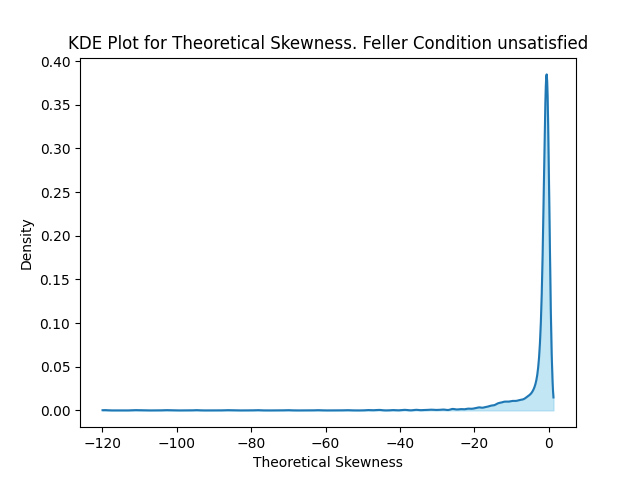
\includegraphics[width=\textwidth]{img/kde_theoretical_skewness_feller_false.png}
        \caption{Theretical Skewness}
    \end{subfigure}
    \hfill
    \begin{subfigure}[b]{0.4\textwidth}
        \centering
        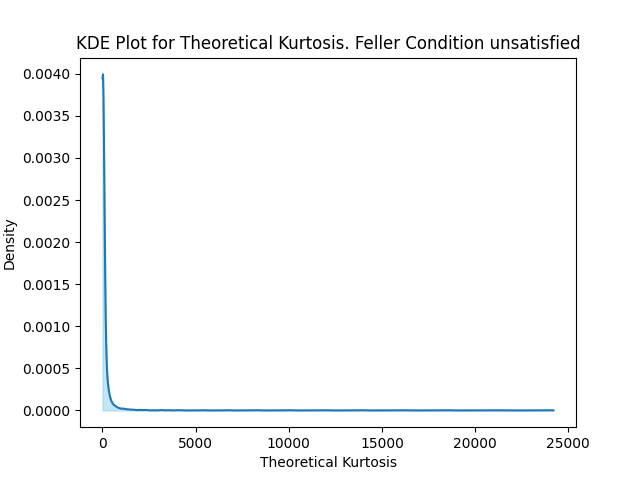
\includegraphics[width=\textwidth]{img/kde_theoretical_kurtosis_feller_false.png}
        \caption{Theoretical Kurtosis}
    \end{subfigure}
    \caption{Kernel density estimation of the theoretical skewness and kurtosis for simulations where the Feller condition is not fulfilled}
    \label{fig:kde_theoretical_skewness_kurtosis_feller_false}
\end{figure}

\section{Investigating the Results for the Gram-Charlier-Expansion with respect to Skewness und Kurtosis}

\begin{figure}
    \centering
    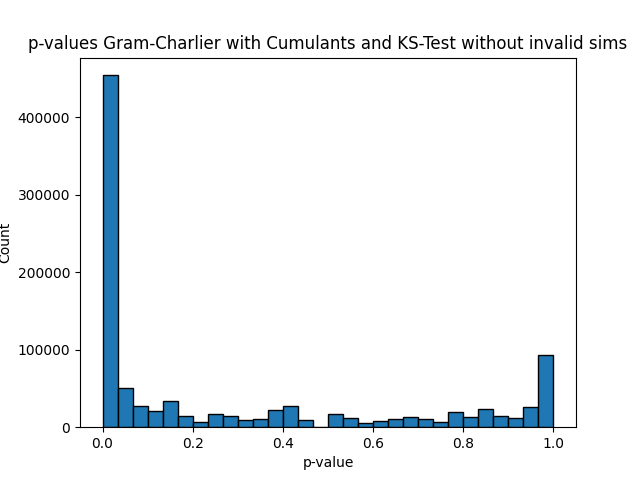
\includegraphics[width=0.8\textwidth]{img/GC_cum_KS_p_value_histogram.png}
    \caption{Distribution of p values of the Kolmogorov-Smirnov-Test for the Gram-Charlier Expansion with Cumulants vs the theoretical density without invalid simulations}
    \label{fig:GC_cum_KS_p_value_histogram}
\end{figure}

Figure \ref{fig:GC_cum_KS_p_value_histogram} shows the distribution of p-values from the Kolmogorov-Smirnov test comparing the Gram-Charlier expansion based on cumulants to the theoretical density. All simulations where the same price appeared more than once have been removed.

A p-value above 5\% indicates that there is no statistically significant difference between the two distributions, meaning that the Gram-Charlier expansion based on cumulants provides an adequate approximation of the theoretical density. However, the results reveal that for some parameter combinations, the approximation does not hold; overall, only 52.48\% of the simulations are able to meet this threshold.

For results on other expansion methods, see Table \ref{tab:KS_p_value_percentage}.

\begin{table}[h]
    \centering
    \begin{tabular}{l|c|c}
        & \textbf{Cumulants} & \textbf{Moments} \\
        \hline
        \textbf{Gram-Charlier} & 52.48\% & 37.35\% \\
        \textbf{GC+}          & 47.63\% & 21.24\% \\
        \textbf{Edgeworth}     & 52.14\% & 36.02\% \\
        \textbf{EW+}          & 47.64\% & 23.27\% \\
        \textbf{Cornish-Fisher} & 35.85\% & 44.90\% \\
        \textbf{Saddlepoint}   & 45.36\% & 40.92\% \\
    \end{tabular}    
    \caption{Percentage of simulations where the p-value of the Kolmogorov-Smirnov-Test against the theoretical density is above 5\%. Invalid simulations are excluded. GC+ and EW+ stand for the Gram-Charlier Expansion with positivity constraint and the Edgeworth Expansion with positivity constraint, respectively.}
    \label{tab:KS_p_value_percentage}
\end{table}

Furthermore, Table \ref{tab:KS_p_value_percentage} shows that expansion methods perform better when based on cumulants rather than moments. Among the examined methods, the Cornish-Fisher expansion and the Saddlepoint approximation, which were briefly discussed in Chapter \ref{sec:literature}, perform the worst. Consequently, these methods, along with all moment-based expansion approaches, will not be considered in further analyses.

The superior performance of the cumulant-based approach can be attributed to its ability to better capture the theoretical skewness and kurtosis of the Heston model compared to the moment-based approach. This is clearly illustrated in Figure \ref{fig:theoretical_vs_real_skewness_kurtosis}. The skewness and kurtosis values proposed by Neuberger \& Payne (\citeyear{neubergerSkewnessStockMarket2021}) are derived directly from raw moments, as described in their original paper.

\begin{figure}
    \centering
    \begin{subfigure}[b]{0.4\textwidth}
        \centering
        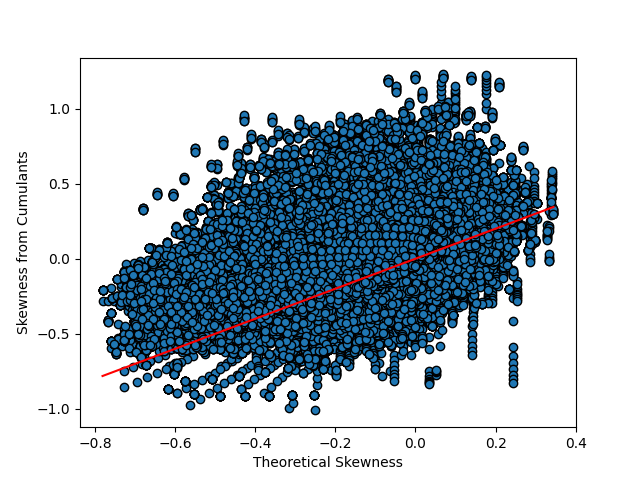
\includegraphics[width=\textwidth]{img/theoretical_skewness_vs_skewness_from_cumulants_feller_condition_true.png}
        \caption{Theretical Skewness vs Skewness from Cumulants}
    \end{subfigure}
    \hfill
    \begin{subfigure}[b]{0.4\textwidth}
        \centering
        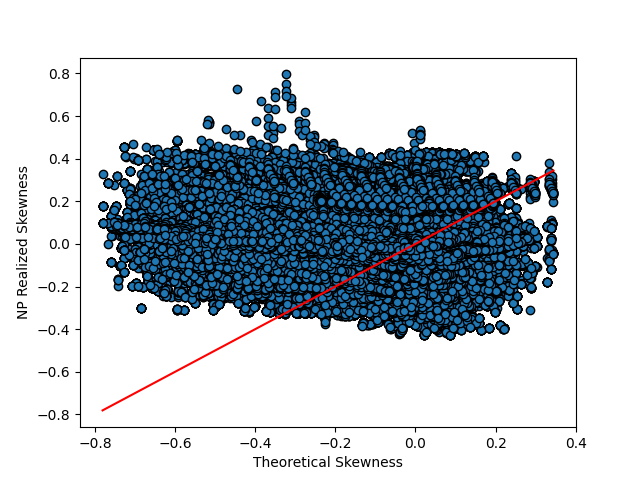
\includegraphics[width=\textwidth]{img/theoretical_skewness_vs_NP_rskewness_feller_condition_true.png}
        \caption{Theoretical Skewness vs Skewness from Neuberger \& Payne (\citeyear{neubergerSkewnessStockMarket2021})}
    \end{subfigure}
    \bigskip % https://tex.stackexchange.com/questions/475149/using-subfigure-and-creating-two-rows-of-figures
    \begin{subfigure}[b]{0.4\textwidth}
        \centering
        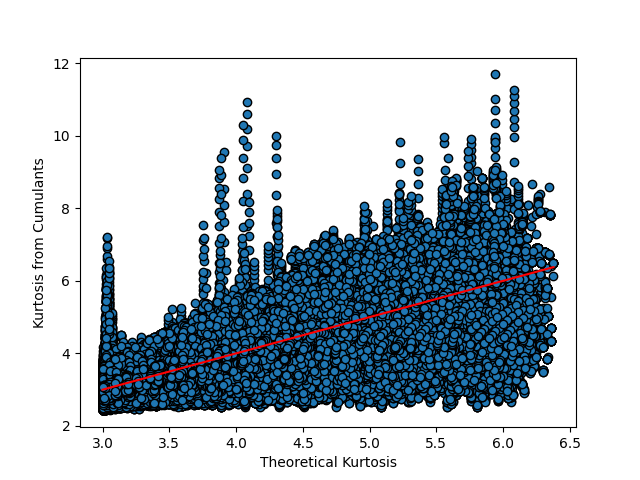
\includegraphics[width=\textwidth]{img/theoretical_kurtosis_vs_kurtosis_from_cumulants_feller_condition_true.png}
        \caption{Theoretical Kurtosis vs Kurtosis from Cumulants}
    \end{subfigure}
    \hfill
    \begin{subfigure}[b]{0.4\textwidth}
        \centering
        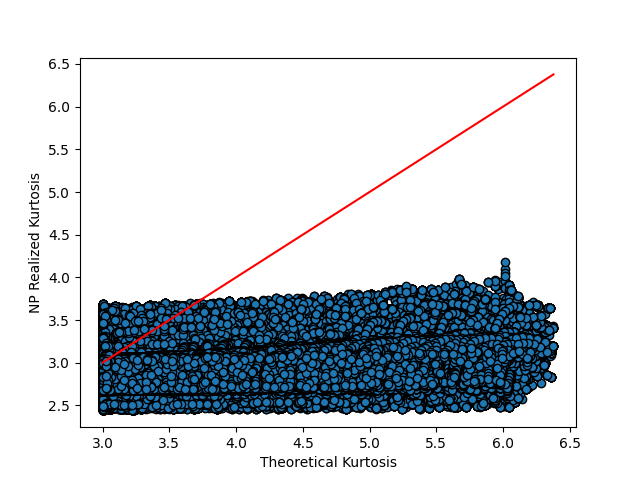
\includegraphics[width=\textwidth]{img/theoretical_kurtosis_vs_NP_rexcess_kurtosis_feller_condition_true.png}
        \caption{Theoretical Kurtosis vs Kurtosis from Neuberger \& Payne (\citeyear{neubergerSkewnessStockMarket2021})}
    \end{subfigure}
    \caption{Comparison of the theoretical skewness and kurtosis with the skewness and kurtosis from the Cumulants and the real skewness and kurtosis from Neuberger \& Payne (\citeyear{neubergerSkewnessStockMarket2021}) for simulations where the Feller condition is fulfilled. Invalid simulations are excluded.}
    \label{fig:theoretical_vs_real_skewness_kurtosis}
\end{figure}

We now examine whether there are correlations between the Heston model parameters and the p-values from the Kolmogorov-Smirnov test. Figure \ref{fig:pairplot_GC_cum_KS_muzero} presents a pair plot illustrating all parameter combinations (excluding $\mu$) and the p-values of the Kolmogorov-Smirnov test for the Gram-Charlier expansion based on cumulants compared to the theoretical density. The more yellow the region, the higher the proportion of p-values above 5\%, indicating a better approximation of the theoretical density by the Gram-Charlier expansion with cumulants.

The color gradients reveal which parameters appear to have an impact. Specifically, $\sigma$, $\kappa$, and $\theta$ seem to influence the quality of the approximation, while $\rho$ appears to have little to no effect. Regardless of how $\rho$ is chosen while holding other parameters fixed, the color distribution remains unchanged. The same applies to $v_0$, which is expected since $v_0$ represents the initial volatility and a burn-in period of three years (out of the 15-year simulation period) was applied to ensure that the unconditional moments and cumulants are not affected by the initial value.

For $\sigma$, the results suggest that lower values lead to better approximations, while higher values of $\kappa$ improve the fit. However, the influence of $\theta$ appears more complex, as there is no clear trend. Generally, higher $\kappa$ values seem to favor higher $\theta$ values, while at low $\sigma$ values, a low $\theta$ is preferable. Figure \ref{fig:GC_cum_KS_3d_p_value_sigma_kappa_theta_muzero} provides a 3D visualization of the relationship between $\sigma$, $\kappa$, and $\theta$ and their impact on the Kolmogorov-Smirnov p-values.

\begin{figure}
    \centering
    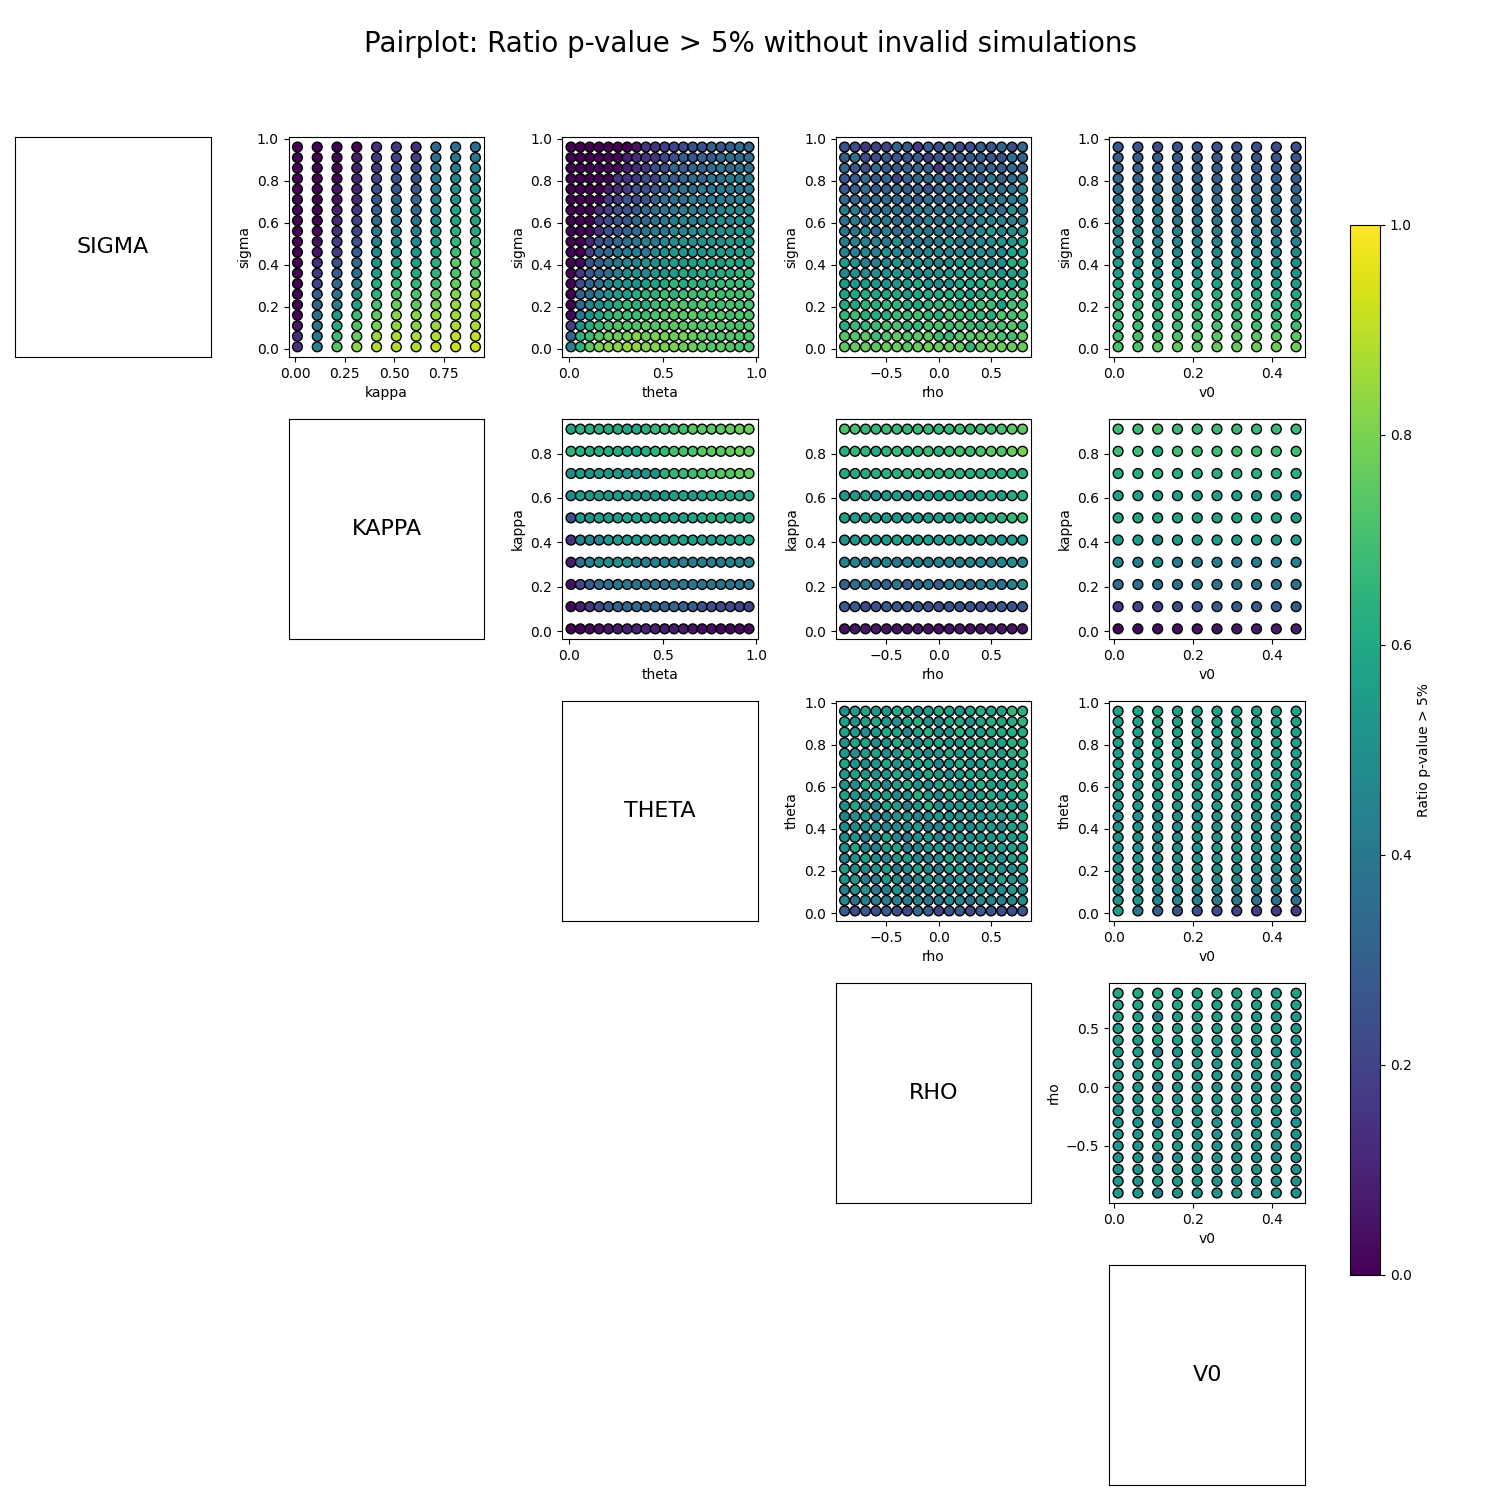
\includegraphics[width=0.8\textwidth]{img/pairplot_GC_cum_KS_muzero.png}
    \caption{Pairplot for each pair of parameters for the Heston Model and the percentage of p values of the Kolmogorov-Smirnov-Test for the Gram-Charlier Expansion with Cumulants vs the theoretical density above 5\%. Invalid simulations are excluded and $\mu=0$.}
    \label{fig:pairplot_GC_cum_KS_muzero}
\end{figure}

\begin{figure}
    \centering
    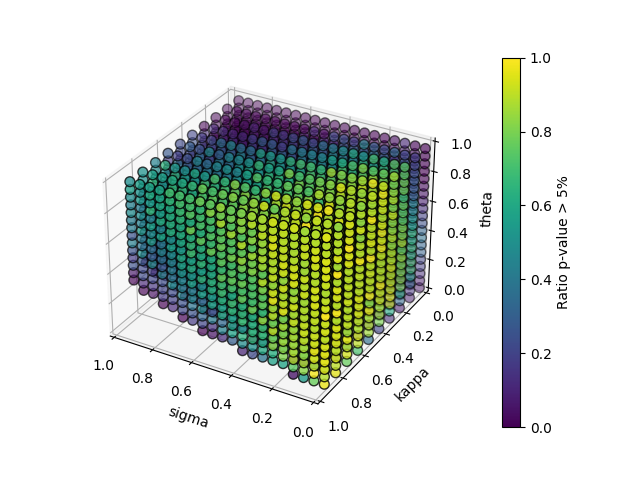
\includegraphics[width=0.8\textwidth]{img/GC_cum_KS_3d_p_value_sigma_kappa_theta_muzero.png}
    \caption{Percentage of simulations where the p-value of the Kolmogorov-Smirnov-Test against the theoretical density is above 5\%. Invalid simulations are excluded. $\mu=0$}
    \label{fig:GC_cum_KS_3d_p_value_sigma_kappa_theta_muzero}
\end{figure}

It is challenging to derive general rules for which parameter combinations lead to good approximations, primarily due to the limitations of graphical visualizations, which cannot effectively represent high-dimensional relationships. To overcome this, we employ classification methods that do not rely on visual representation, such as logistic regression and random forests.

For this analysis, all valid simulations were used and split into 80\% training data and 20\% test data. The independent variables $X$ are the Heston model parameters, while the dependent variable $y$ indicates whether the Kolmogorov-Smirnov p-value exceeds 5\%. The dataset is imbalanced, with 60.98\% of simulations yielding a p-value above 5\%. The logistic regression model achieves an accuracy of 79.53\%, while the random forest model, consisting of 100 decision trees, reaches 91.59\% accuracy. The precision for $y = 1$ is 82\% for logistic regression and 92\% for the random forest model.

Precision is particularly relevant in this context, as it represents the proportion of true positives among all predicted positives. A low precision would imply that parameter combinations unsuitable for the Gram-Charlier approximation are mistakenly classified as suitable. In a financial context, where such approximations might be used to price securities, incorrect classifications could lead to substantial financial losses.

Examining the logistic regression coefficients (Table \ref{tab:logistic_regression_coefficients}) and the feature importance scores from the random forest model (Figure \ref{fig:feature_importances}) reveals that $\sigma$ is by far the most influential parameter. Both $\theta$ and $\kappa$ are also important, but the models disagree on which of the two has a stronger impact. The role of $\rho$ is also unclear—it is insignificant in logistic regression but influential in the random forest model. Conversely, $\mu$ and $v_0$ play no significant role. All parameters included in the models are statistically significant.

\begin{table}
    \centering
    \begin{tabular}{l|c|c|c|c}
        \textbf{Parameter} & \textbf{Coefficient} & \textbf{Standard Error} & $z$ & $\mathbb{P}>\vert z\vert$ \\
        \hline
        const & -0.8708 & 0.010 & -84.332 & 0.000 \\
        $\mu$ & -1.2841 & 0.111 & -11.568 & 0.000 \\
        $\sigma$ & -7.2015 & 0.017 & -429.506 & 0.000 \\
        $\kappa$ & 4.4584 & 0.014 & 318.689 & 0.000 \\
        $\theta$ & 3.0120 & 0.013 & 237.146 & 0.000 \\
        $\rho$ & 0.4219 & 0.005 & 78.359 & 0.000 \\
        $v_0$ & -0.0728 & 0.019 & -3.765 & 0.000
    \end{tabular}
    \caption{Coefficients of the logistic regression}
    \label{tab:logistic_regression_coefficients}
\end{table}

\begin{figure}
    \centering
    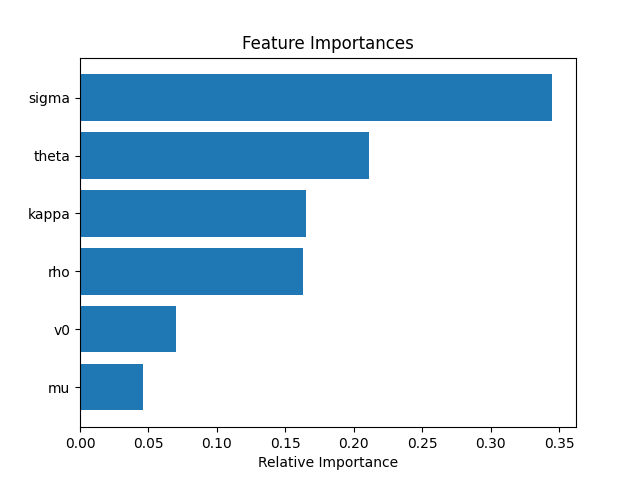
\includegraphics[width=0.8\textwidth]{img/feature_importances.png}
    \caption{Feature Importances of the Random Forest}
    \label{fig:feature_importances}
\end{figure}

\section{Comparing the Expansion Methods}

\subsection{General Approximation}
So far, we have analyzed the Gram-Charlier expansion from multiple perspectives. However, an important question remains: Are expansion methods even worth using? To answer this, we first examine whether adding the third and fourth cumulants improves the results, specifically in relation to the theoretical skewness and kurtosis.

As a baseline model, we use the normal distribution, which relies only on the first two cumulants—the mean ($\mu$) and variance ($\sigma^2$). This allows us to compare whether incorporating higher-order cumulants provides a meaningful advantage. The results of this comparison are shown in Figure \ref{fig:gc_vs_no_theoretical_skewness_kurtosis}.

The findings indicate that using a more complex expansion method than the normal distribution is beneficial, as the approximation improves significantly for given levels of skewness and kurtosis.

\begin{figure}
    \centering
    \begin{subfigure}[b]{0.4\textwidth}
        \centering
        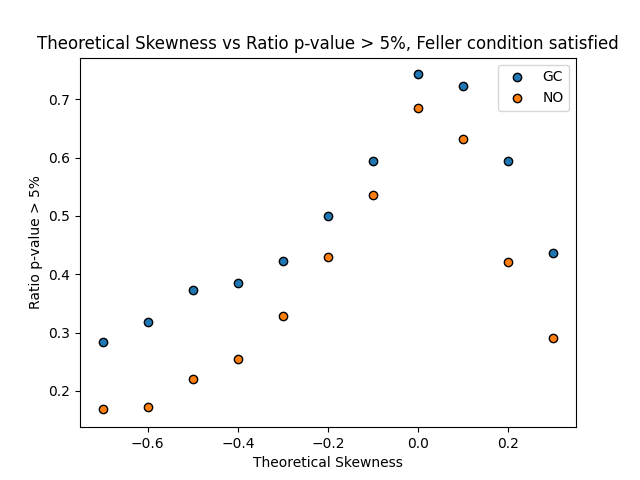
\includegraphics[width=\textwidth]{img/theoretical_skewness_vs_ratio_feller_condition_true.png}
        \caption{Theretical Skewness}
    \end{subfigure}
    \hfill
    \begin{subfigure}[b]{0.4\textwidth}
        \centering
        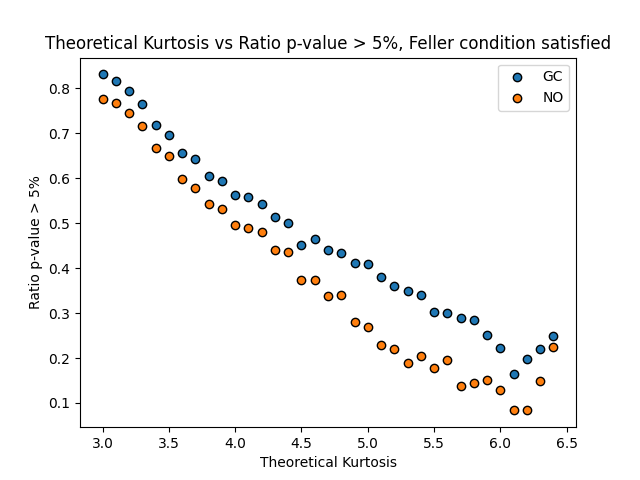
\includegraphics[width=\textwidth]{img/theoretical_kurtosis_vs_ratio_feller_condition_true.png}
        \caption{Theoretical Kurtosis}
    \end{subfigure}
    \caption{Ratio of simulations where the p-value of the Kolmogorov-Smirnov-Test against the theoretical density is above 5\% in relation to the theoretical skewness and kurtosis. GC stands for the Gram-Charlier-Expansion while NO stands for the Normal Distribution. Feller condition is fulfilled.}
    \label{fig:gc_vs_no_theoretical_skewness_kurtosis}
\end{figure}

\begin{figure}
    \centering
    \begin{subfigure}[b]{0.4\textwidth}
        \centering
        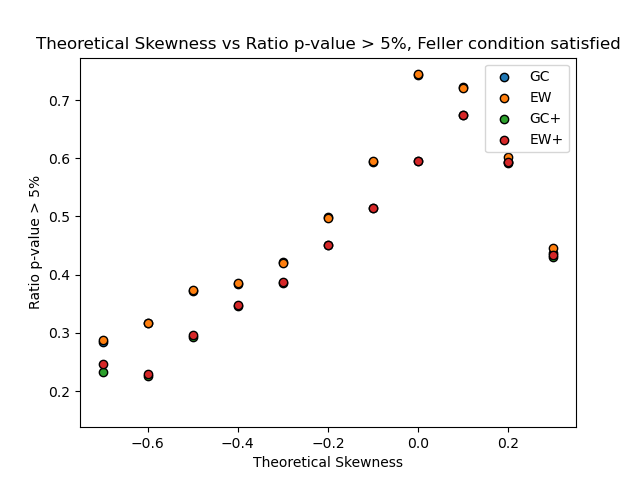
\includegraphics[width=\textwidth]{img/theoretical_skewness_vs_ratio_gc_ew_feller_condition_true.png}
        \caption{Theretical Skewness}
    \end{subfigure}
    \hfill
    \begin{subfigure}[b]{0.4\textwidth}
        \centering
        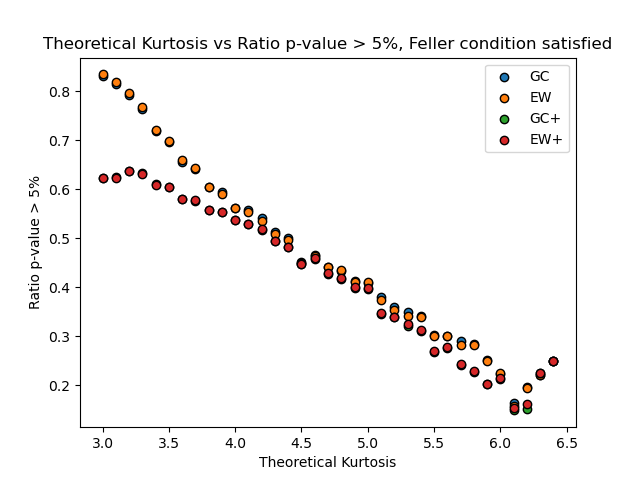
\includegraphics[width=\textwidth]{img/theoretical_kurtosis_vs_ratio_gc_ew_feller_condition_true.png}
        \caption{Theoretical Kurtosis}
    \end{subfigure}
    \caption{Ratio of simulations where the p-value of the Kolmogorov-Smirnov-Test against the theoretical density is above 5\% in relation to the theoretical skewness and kurtosis. GC stands for the Gram-Charlier-Expansion, EW for the Edgeworth-Expansion. A $+$ behind the Expansion denotes the variant with positivity constraints. Feller condition is fulfilled.}
    \label{fig:gc_vs_ew_theoretical_skewness_kurtosis}
\end{figure}

A similar pattern emerges when comparing the Gram-Charlier expansion and the Edgeworth expansion, along with their positivity-constrained variants. The results, shown in Figure \ref{fig:gc_vs_ew_theoretical_skewness_kurtosis}, indicate that positivity-constrained variants perform significantly worse. This decline in performance is due to the distortion effect introduced by the positivity constraint.

Moreover, no specific Heston model parameter dependencies were found where positivity-constrained expansions outperform their unconstrained counterparts. However, this is largely because the chosen parameter combinations for the simulations never result in theoretical skewness or kurtosis values that exceed the validity range of the expansion methods. As a result, the positivity constraints never actually prevent negative density values, which would otherwise invalidate the expansion as a proper density function.

To investigate cases where the Edgeworth expansion provides a better approximation, we search the database for parameter combinations where:
\begin{enumerate}
    \item The p-value from the Kolmogorov-Smirnov test is higher for the Edgeworth expansion than for the Gram-Charlier expansion.
    \item The p-value for the Edgeworth expansion is above 5\%, while the p-value for the Gram-Charlier expansion is below 5\%.
\end{enumerate}
A total of 2,866 such parameter combinations were identified out of 501,713 possible cases (after filtering out invalid simulations), representing only 0.57\% of all simulations. This suggests that the Edgeworth expansion is not a better alternative to the Gram-Charlier expansion for the Heston model.

\subsection{Approximation of the Tails}
To compare the tails of the distributions, we use the Anderson-Darling test. Additionally, we attempted a comparison using the Hill estimator to estimate the tail index. However, it was not possible to identify a plateau in the Hill plot, which suggests that the tails are not sufficiently fat, as seen in distributions like the Pareto distribution. This is a critical requirement for the Hill estimator to be applicable.

One might expect that using a test that is more sensitive to the tails, such as the Anderson-Darling test, would yield different results compared to previous tests. However, the comparison between Figure \ref{fig:pairplot_GC_cum_AD_muzero} and Figure \ref{fig:pairplot_GC_cum_KS_muzero} reveals practically no difference. This suggests that the Gram-Charlier expansion based on cumulants provides a good approximation of the tails as well.

\begin{figure}
    \centering
    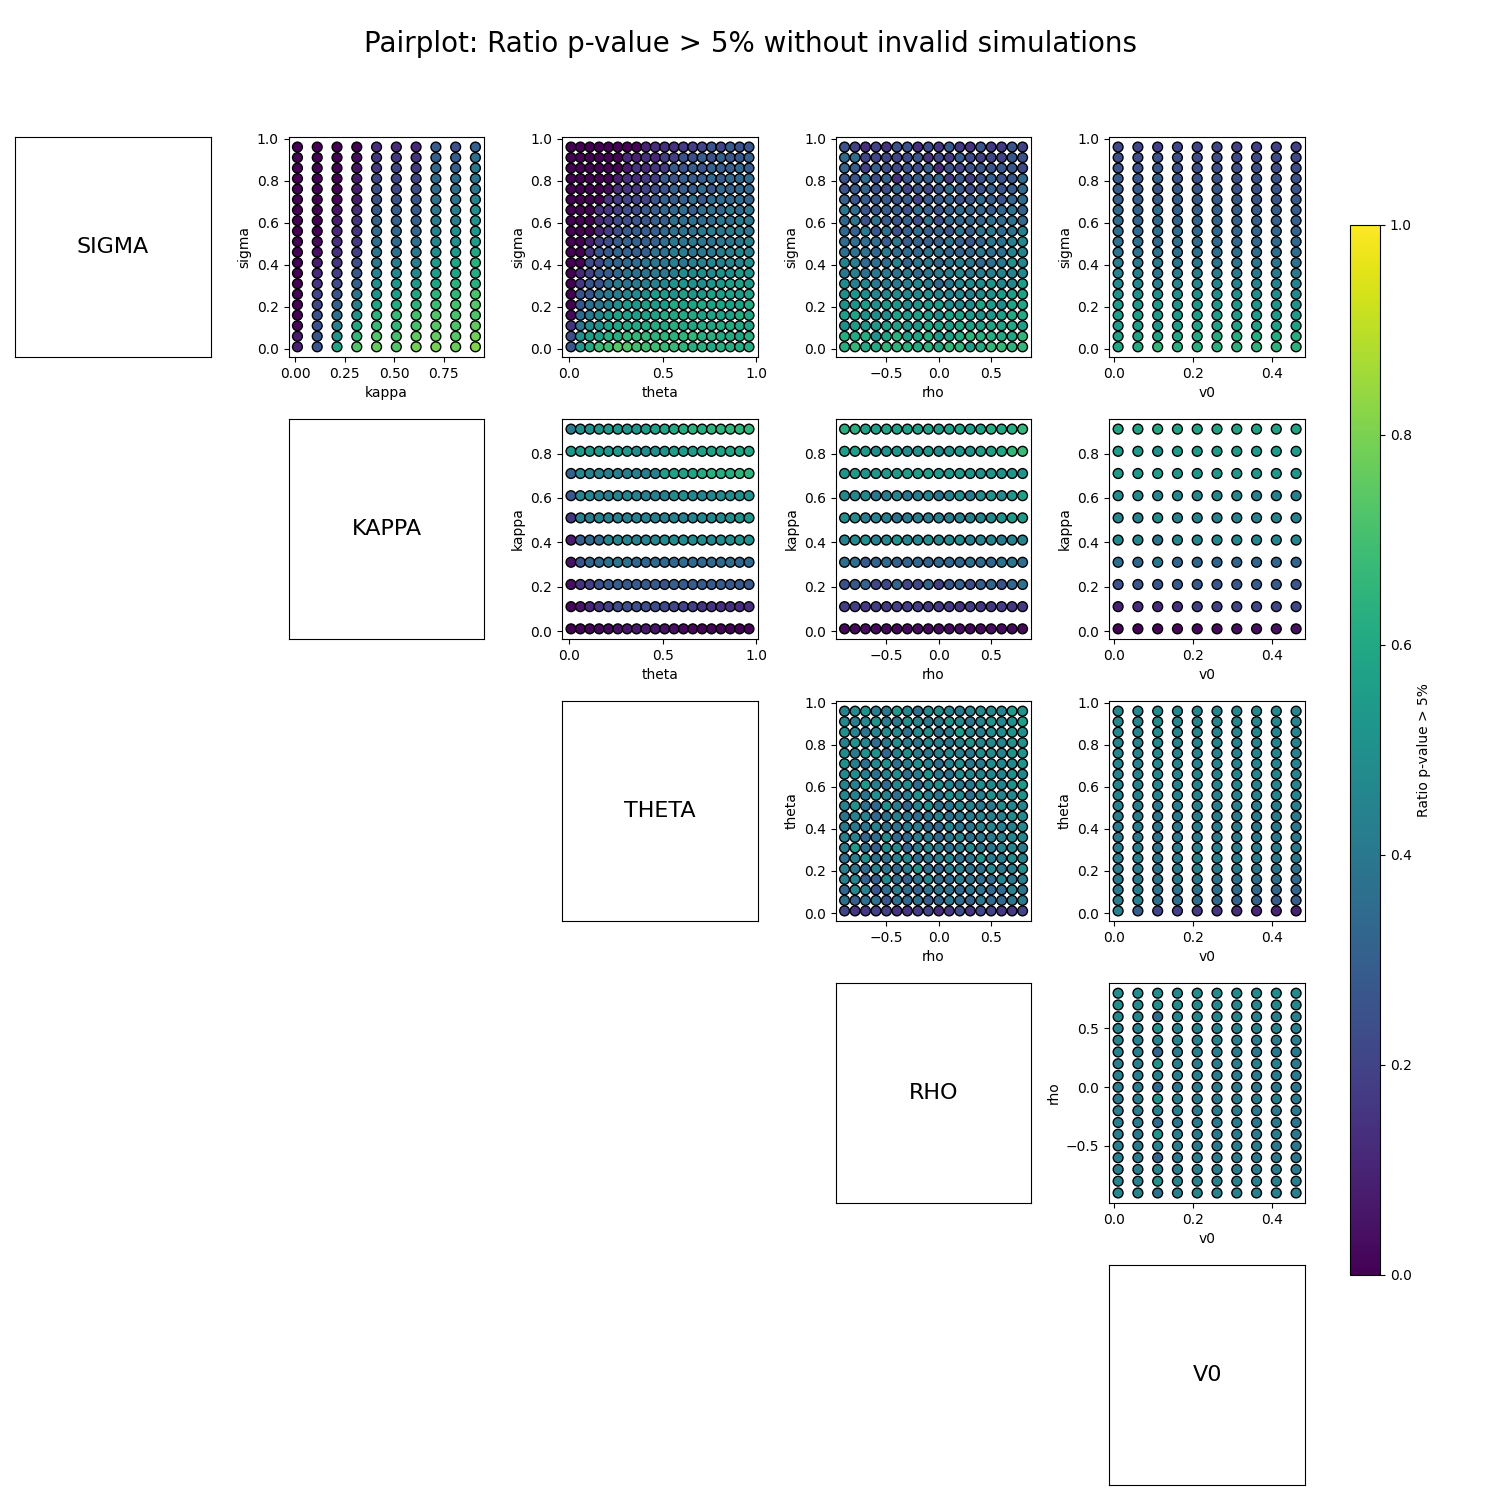
\includegraphics[width=0.8\textwidth]{img/pairplot_GC_cum_AD_muzero.png}
    \caption{Pairplot for each pair of parameters for the Heston Model and the percentage of p values of the Anderson-Darling-Test for the Gram-Charlier Expansion with Cumulants vs the theoretical density above 5\%. Invalid simulations are excluded and $\mu=0$.}
    \label{fig:pairplot_GC_cum_AD_muzero}
\end{figure}